\documentclass[pdftex,10pt,b5paper,twoside]{book}
\usepackage[utf8]{inputenc}
\usepackage[toc,page]{appendix}
\usepackage[T1]{fontenc}
\usepackage[lmargin=25mm,rmargin=25mm,tmargin=27mm,bmargin=30mm]{geometry}
\usepackage[]{todonotes}
\usepackage{import}
\usepackage{graphicx}
\usepackage{amsmath}
\usepackage[sc]{mathpazo}
\usepackage{bm}
\usepackage{nomencl}
\usepackage{gensymb}
\usepackage{rotating}
\usepackage{etoolbox}
\usepackage{hyperref}
\usepackage{titlesec}
\usepackage{subfig}
\usepackage{subfiles}
\usepackage{multirow}
\usepackage{setspace}
\usepackage{fancyhdr}
\usepackage{enumitem}
\usepackage{pdfpages}
\usepackage{pgf,tikz,pgfplots}
\usepackage{mathrsfs}
\usepackage[noend]{algpseudocode}
\usetikzlibrary{arrows}
\pgfplotsset{compat=1.15}
\usepackage{mathrsfs}
\usepackage{tabularx}
\usepackage[ruled,vlined]{algorithm2e}
\usepackage{algcompatible}
\usetikzlibrary{arrows}
%\definecolor{xdxdff}{rgb}{0.49019607843137253,0.49019607843137253,1}
%\definecolor{ffqqqq}{rgb}{1,0,0}
%\definecolor{ududff}{rgb}{0.30196078431372547,0.30196078431372547,1}
%\definecolor{uuuuuu}{rgb}{0.26666666666666666,0.26666666666666666,0.26666666666666666}

\setcounter{tocdepth}{2}
\setcounter{secnumdepth}{2}
\setlength\parindent{0pt}
\numberwithin{equation}{chapter}
\newcommand{\respage}[1]{\pagenumbering{#1}\setcounter{page}{1}}
\renewcommand{\listtablename}{Tables}
\newcommand{\figtable}[2]{
	\subfloat[]{
    	\includegraphics[scale=#1]{#2}
    }
}

%math
\newcommand{\at}[2][]{#1|_{#2}}
\newcommand{\pr}{P}
\newcommand{\range}{r}
\newcommand{\zeros}[2]{\bm{0}_{#1\times#2}}
\newcommand{\partialdiff}[2]{\frac{\partial #1}{\partial #2}}
\newcommand\numberthis{\addtocounter{equation}{1}\tag{\theequation}}
\newcommand{\omgbe}{\bm{\omega_{be}^b}}
\newcommand{\omgie}{\bm{\omega}_{ie}^e}
\newcommand{\half}{\frac{1}{2}}
\newcommand{\fimu}{\bm{f}_{IMU}^b}
\newcommand{\rot}[2]{\bm{R}^#1_#2}
\newcommand{\eb}[1]{\bm{#1}^e_{be}}
\newcommand{\ebd}[1]{\bm{\dot{#1}}^e_{be}}
\newcommand{\bmeps}{\bm{\varepsilon}}
\newcommand{\bmeta}{\bm{\eta}}
\newcommand{\eye}[1]{\bm{I}_{#1\times#1}}
\newcommand{\xkn}{\hat{\bm{x}}_{k+1}}
\newcommand{\xk}{\hat{\bm{x}}_k}
\newcommand{\xkp}{\hat{\bm{x}}_{k-1}}
\newcommand{\Pkn}{\bm{P}_{k+1}}
\newcommand{\Pk}{\bm{P}_k}
\newcommand{\atk}[1]{\bm{#1}_k}
\newcommand{\atkn}[1]{\bm{#1}_{k+1}}
\newcommand{\atkp}[1]{\bm{#1}_{k-1}}
\newcommand{\norm}[1]{\left\lVert#1\right\rVert}
\newcommand{\cps}{c(\psi)}
\newcommand{\cth}{c(\theta)}
\newcommand{\cph}{c(\phi)}
\newcommand{\sps}{s(\psi)}
\newcommand{\sth}{s(\theta)}
\newcommand{\sph}{s(\phi)}

%State vector
\newcommand{\pos}{\hat{\bm{p}}^e_{be}}
\newcommand{\vel}{\hat{\bm{v}}^e_{be}}
\newcommand{\ba}{\hat{\bm{b}}_a}
\newcommand{\bias}{\hat{\beta}_{gps}}
\newcommand{\biasdot}{{\hat{\beta}_d}}
\newcommand{\biasglo}{\hat{\beta}_{glonass}}

\newcommand{\posd}{\dot{\hat{\bm{p}}}^e_{be}}
\newcommand{\veld}{\dot{\hat{\bm{v}}}^e_{be}}
\newcommand{\biasd}{\dot{\hat{\beta}}_{gps}}
\newcommand{\biasdotd}{\dot{\hat{\beta}}_d}
\newcommand{\biasglod}{\dot{\hat{\beta}}_{glonass}}

%\AtBeginEnvironment{algorithm}{\algoequations}
%\AtEndEnvironment{algorithm}{\restoreequations}
%\newcounter{algosavedequation}
%\newcommand{\algoequations}{%
%  \setcounter{algosavedequation}{\value{equation}}%
%  \setcounter{equation}{0}%
%  \renewcommand{\theequation}{Alg\thealgocf.\arabic{equation}}%
%}
%\newcommand{\restoreequations}{%
%  \setcounter{equation}{\value{algosavedequation}}%
%}
%\newcommand{\skew}[1]{\bm{S(#1)}} \todo{Fix}

\title{Master drafts}
\author{Øyvind Aukrust Rones}
\date{November 2018}

\begin{document}
\todo{Change document structure (paragraph should add a new line)}
\maketitle

\listoftodos
\subimport{Preliminaries/}{frontpage.tex}
\pagenumbering{roman}
\subimport{Preliminaries/}{nomenclature.tex}
\tableofcontents
\listoffigures
\listoftables

\chapter{Introduction}
\respage{arabic}
    %GNSS long term accuracy. Complements imu
%Example of dune tightly coupled with rtklib running separately
%All of these approaches work offline and as such there is a need for a working online implementation.
%Low frequency of GNSS does not capture high dynamics
\newpage
\chapter{Theoretical background}
    \graphicspath{{Theory/}}
This chapter presents the background information that this thesis is built on. An overview of GNSS is given, followed by a look into the integration of INS and GNSS and ending with a quick overview of the major software packages used in the implemented system. 

\section{Global Navigation Satellite Systems}
    \todo{reference prosjektoppgave}
    \subimport{Theory/}{gnssNew.tex}

\section{Integrating INS and GNSS}
    \subimport{Theory/}{integration.tex}

\section{Software packages}
    \subimport{Theory/}{software-packages.tex}
%Structure
    % 1 - INS
    % 2 - GNSS
    % 3 - Integration
    
%x Theory
%x  - GNSS (raskt renskrevet fra prosjektoppgave)
%x  - Integration
%x     1 - Motivation
%x         + Improving state estimation
%x     2 - Architectures
%x         + Loose
%x         + Tight
%x         + Ultra tight
%x         + Feedback vs open loop
%x     3 - Kalman filter
%x         + KF / EKF
%x           - Indirect implementation
%x               - Orientations state minimal. No over-parametrization
%x               - Operating close to the origin. Far away from singularities
%x               - Always small. Second-order products negligible
%x               - Error dynamics are small. All large dynamics already in nominal state. Can apply
%x               - corrections at a lower rate than predictions 
%x               - \cite{sola2017quaternion}
%x           - MEKF
%x               - Maintains quaternion unit length
%x     4 - Parametrizations
%x         + Vector-angle
%x         + Euler
%x         + Quaternion (Linear diff. eq. No EKF divergence)
%x         + Gibbs
%x         + Modified Rodrigues
    
\newpage
\chapter{Implementation}
    \graphicspath{{Implementation/}}
\label{ch:implementation}

%%% INTRO %%%
This chapter presents a tightly coupled extended Kalman filter estimating position and velocity from acceleration, pseudo-range and Doppler shift measurements. A mathematical derivation of the filter model is shown first, followed by an overview of the DUNE implementation. The hardware running the implementation is then presented before the chapter ends with an overview of the testing and tuning process.

\section{Extended Kalman filter}
\label{sec:imp:ekf}
    \subimport{Implementation/}{EKF.tex}

\section{DUNE implementation}
    \subimport{Implementation/}{Dune.tex}

%\section{Testing and tuning}
%    \label{sec:imp:simulator}
%    \subimport{Implementation/}{Simulators.tex}

\section{Embedded Platform}
    \subimport{Implementation/}{Hardware.tex}

\section{Testing}
    \subimport{Implementation/}{testing.tex}
        

%introduction
%   + ?MavProxy
%   Hardware and control
%   + Mention hardware package: BBB, Pixhawk, ArduPilot

%%   Actual implementation  %%
%   Simulators for testing
%       + SITL, JSBSim, Flightgear, Simple GNSS
%   RTKLIB
%       + Play back file (no waiting for eph), read serial
%       + Apply corrections
%       + ?svr-struct
%       + Dispatch as IMC to DUNE
%       + Gotta add cmake
%   EKF
%       + IMC messages, ground truth, imu, gnss
%       + Tightly coupled, indirect, general equations
%       + Model details (loads of equations)
%           - State model, Error state model, Measurement model, noise model
%           - Two possibilities for integrating attitude error to nominal state
%           
%   Installing on BBB
%       + Glued
%           - Docker, partition disk, sd-card
%       + Dune
%           - Cross compiling
        
%Structure simulators
    % 1 - GNSS 
    %       possible to set frequency. Delay between samples
    %       range and range rate
    % 2 - Flightgear
    %     + Changing of ardupilot code (use flightgear simulator instead of AP-interface for better imu precision)
    % 3 - JSBSim?
    
    
%% Questions
% What is SITL?
%   ardupilot.org/dev/docs/sitl-simulator-software-in-the-loop.html
%   http://ardupilot.org/dev/_images/ArdupilotSoftwareintheLoopSITL.jpg
%   Run ardupilot without any hardware, directly on PC (opposed to HIL)
%   AP-SIL can simulate a bunch of random vehicles
%   Start SITL simulator: sim_vehicle.py
%   "When running in SITL the sensor data comes from a flight dynamics model in a flight simulator."
%   "SITL outputs FlightGear compatible state information on UDP port 5503"
%   Set sitl to auto to call takeoff command, then arm. Can set to different mode after

%MAVPROXY?
%   "A UAV ground station software package for MAVLink based systems"
%   ?Mission planner console. Battery status and stuff like that?
%   Supports different modes: Guided, land, auto..
%   Graph takeoff: gtakeoff

% How does Neptus get SITL-data?
%   ?Listening to ports
%   ?SITL outputs FlightGear compatible state information on UDP port 5503
% What's the difference between flightgear and jsbsim?
\newpage
\chapter{Results}
    This section presents the results of running the system described in section \ref{ch:implementation}, with the goal of investigating performance of the EKF with real, raw data.\\ 


% Drawn path used as reference for lat lon
% px used as imperfect reference with regards to height because of extra sensors
% 
The tests were carried out taking the payload by foot along a path drawn up before testing. The path was laid along a number of small roads to make it easy to follow and thus minimize the difference between it and the actual path taken. This is therefore used as a reference for position in the horizontal plane as latitude and longitude coordinates. Additionally, position, as well as velocity, is compared with the separate PixHawk estimates. The RTKLIB position estimates are included as well.\\

\section{Stationary tests}

\section{Dynamic tests}
    \subsection{GNSS only}
    \begin{figure}
        \centering
        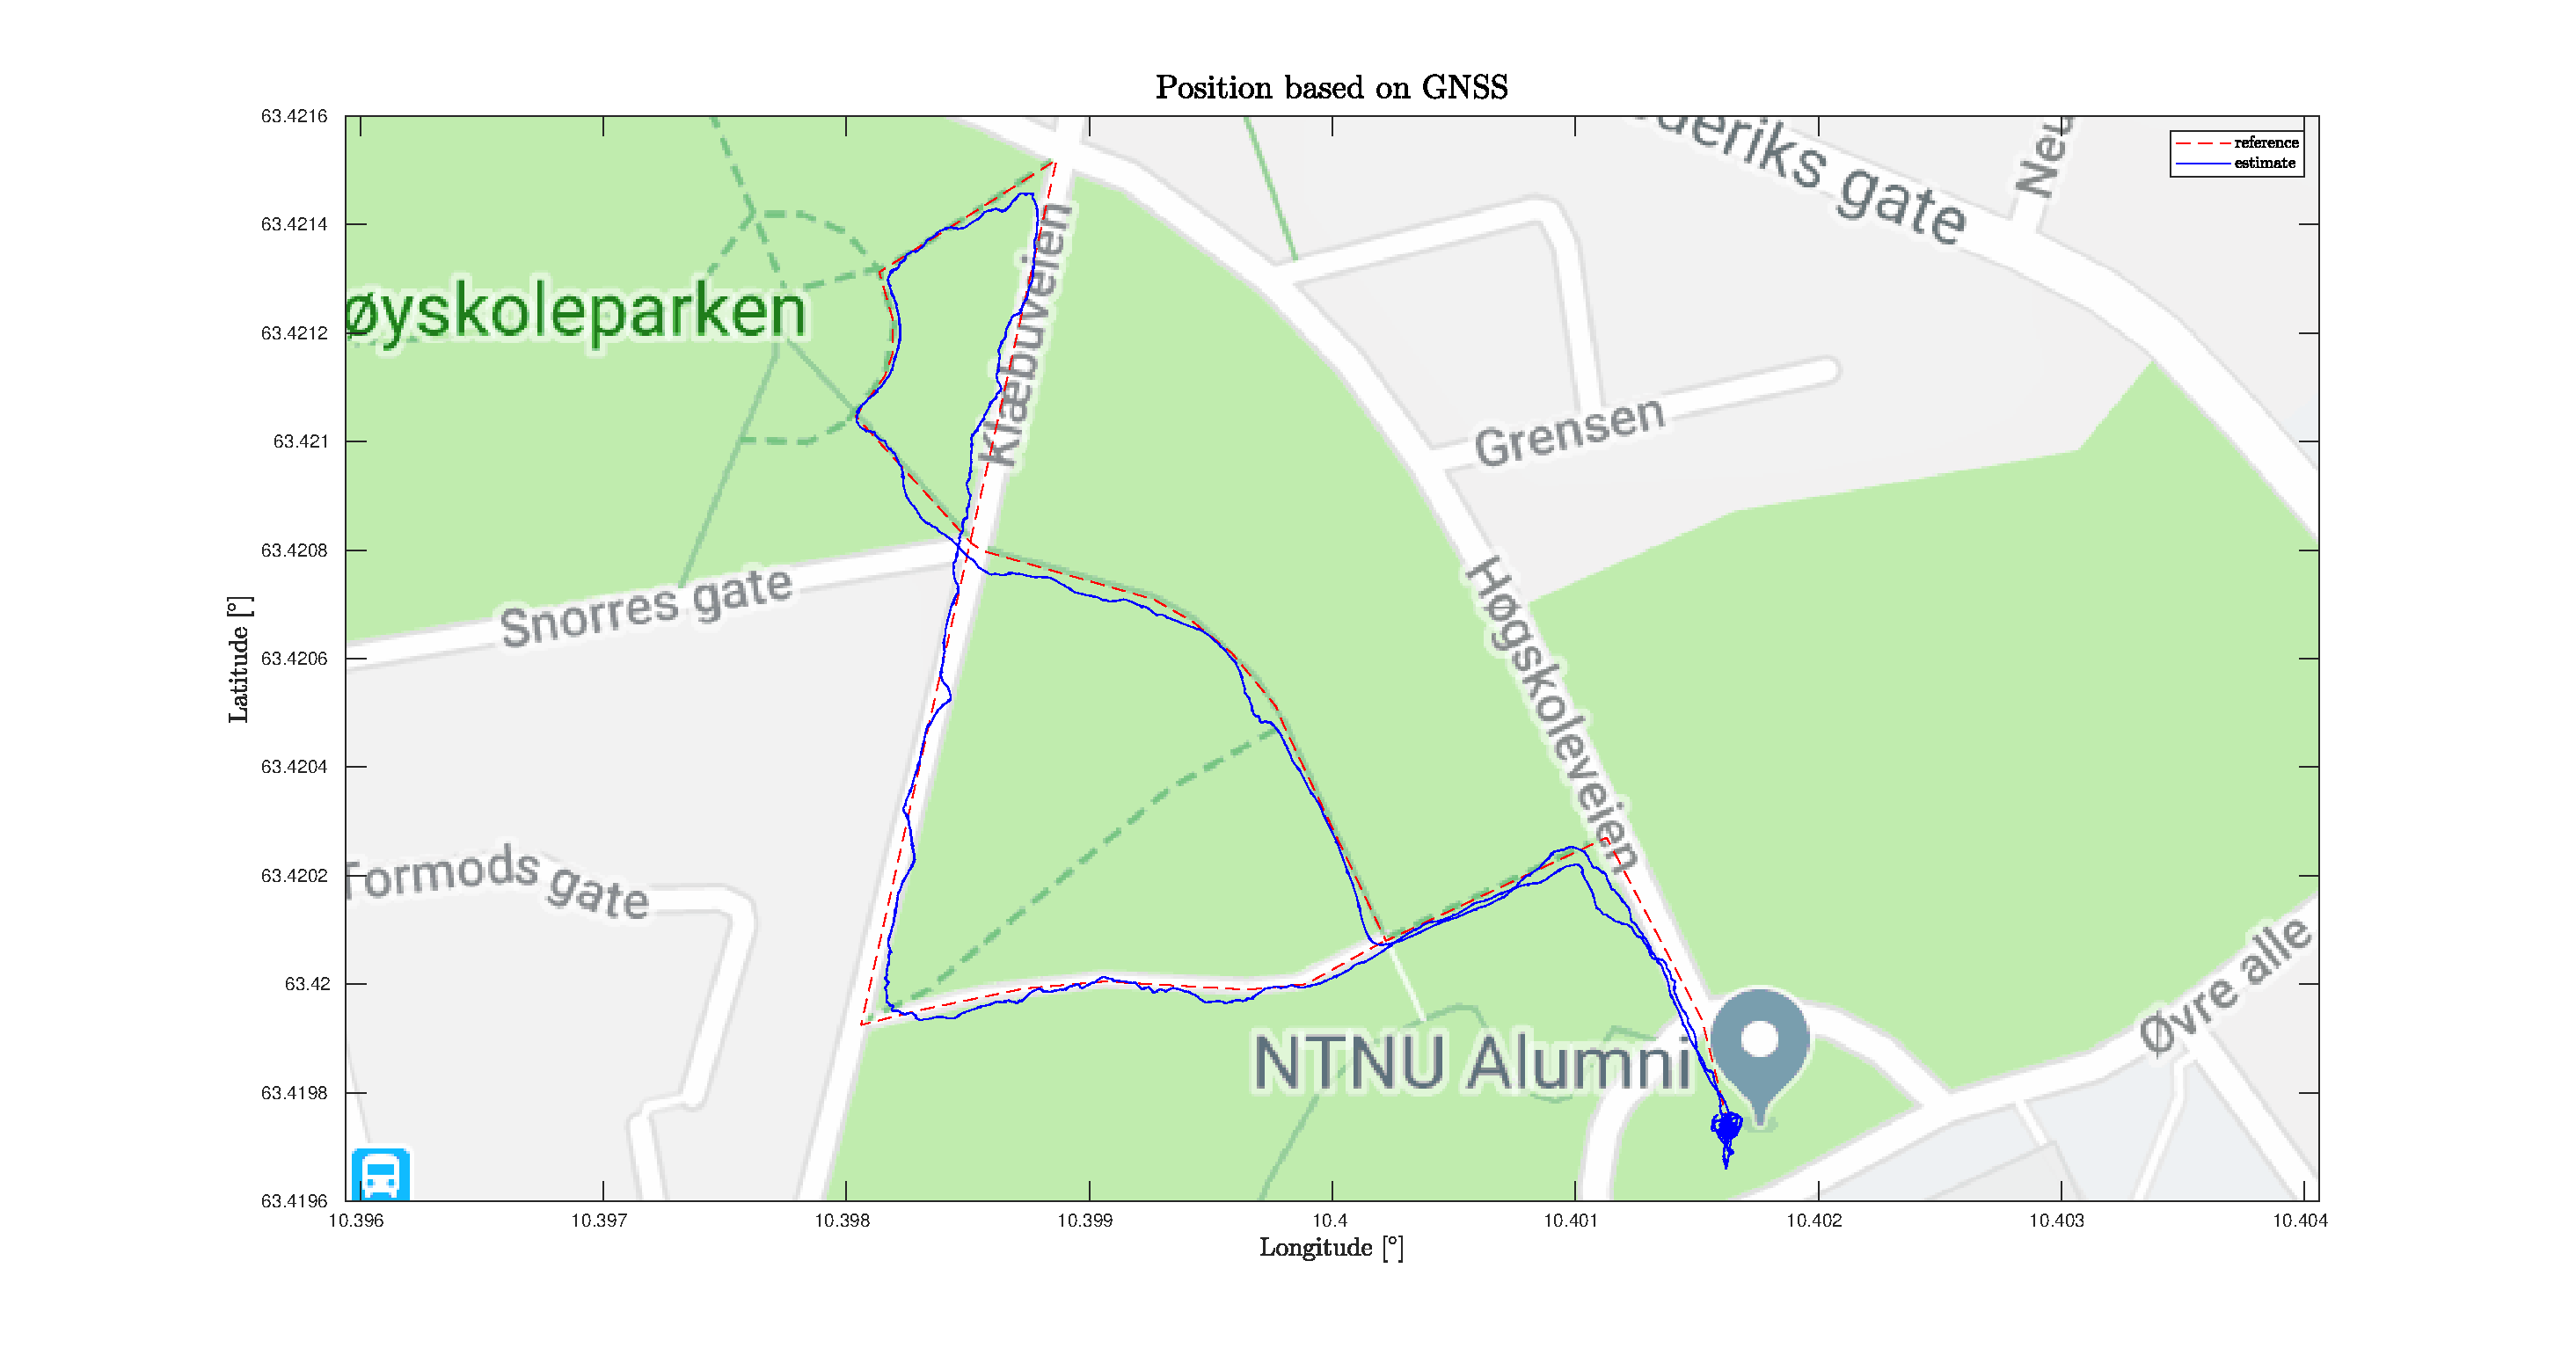
\includegraphics[scale=0.3]{Results/Images/gnss-only.eps}
        \caption{Position estimate based on GNSS measurements only}
        \label{fig:test-gnss}
    \end{figure}
    
    
    
    
    
    
    
    
    
    
    
    
    
    
    
    
    
    
    
    
    
    
    
    
    
    
    
    
    
    
    
    
    
    
    
    
    
    
%\begin{comment}
%\section{Performing the tests}
%To compare the MEKF with other systems several tests were devised, keeping in mind known %limitations of each of the systems. 
%\todo{Describe tests and thoughts behind them}

%\begin{table}[!htbp]
%\caption{List of tests}
%\label{tab:tests}
%    \begin{tabular}{|l|l||p{5cm}|}
%        \hline
%        \textbf{Tested systems} & \textbf{Test description} & \textbf{Expected result}\\
%        \hline
%        Coupled/uncoupled & Circular pattern & The MEKF should show an increase in %precision compared to the     single GNSS solution.\\
%        \hline
%        Indirect/direct filter &  Highly dynamic zigzag motion & The MEKF should follow %the quickly changing     state better than the direct filter.\\
%        \hline
%        The full system & Straight line motion/square pattern & The MEKF should generally %perform better than     the other systems\\
%        \hline
%    \end{tabular}
%\end{table}%
%
%\todo{Describe test environment}
%\missingfigure[]{Ottobil}

%Structure
    % 1 - Introduction
    %     + Test location
    %     + List of compared systems
    % 2 - Performing the tests
    %     + Description of how the tests were performed (waited for steady state..)
    % 3 - Actual results
    %     + Graphs, tables, rms
    %     + 
    
\todo{Log cpu usage}

%\end{comment}

%This chapter presents the experimental results from running the system described in chapter \ref{ch:implementation}. A base station with a setup similar to the described system was set up, and the results are compared to the RTK solution of RTKLIB, as well as the internal PixHawk state estimate.
\newpage
    
\graphicspath{{Appendices/}}
\begin{appendices}
\chapter{Reference frames}
    \subimport{Appendices/}{reference-frames.tex}

\chapter{Hardware}
    \subimport{Appendices/}{hardware.tex}
    
\chapter{Atmospheric models}
    \subimport{Appendices/}{klobuchar.tex}
\end{appendices}
    
\bibliographystyle{abbrv}
\bibliography{bibliography.bib}
    
\end{document}


%x Introduction
%x  - Frontpage
%x  - Abstract
%x  - Sammendrag
%x  - List of figures/tables
%x  - Nomenclature/abbreviations

%x Theory
%x  - GNSS (raskt renskrevet fra prosjektoppgave)
%x  - Integration
%x     1 - Motivation
%x         + Improving state estimation
%x     2 - Architectures
%x         + Loose
%x         + Tight
%x         + Ultra tight
%x         + Feedback vs open loop
%x     3 - Kalman filter
%x         + KF / EKF
%x           - Indirect implementation
%x               - Orientations state minimal. No over-parametrization
%x               - Operating close to the origin. Far away from singularities
%x               - Always small. Second-order products negligible
%x               - Error dynamics are small. All large dynamics already in nominal state. Can apply
%x               - corrections at a lower rate than predictions 
%x               - \cite{sola2017quaternion}
%x           - MEKF
%x               - Maintains quaternion unit length
%x         + Nonlinear observer(?)
%x     4 - Parametrizations
%x         + Vector-angle
%x         + Euler
%x         + Quaternion (Linear diff. eq. No EKF divergence)
%x         + Gibbs
%x         + Modified Rodrigues
%x         + Cayley parameters?
    
% Implementation
%x  - Toolchain
%x     1 - Dune, Neptus, IMC
%x     2 - Glued
%x     3 - RTKLIB
%x  - Hardware
%x     1 - Beaglebone black
%x     2 - Shield 3.0
%x     3 - GNSS receiver
%x  - Simulators
%x     1 - GNSS simulator
%x     2 - Flightgear
%x         + Changing of ardupilot code
%x  - Full system
%x     1 - EKF method description
%x         + Because the expected error state is always zero except between a measurement correction and              the injection of the error in to the nominal state, followed by a reset, there is no poin                in actually implementing the propagation of the error state. The covariance of the error is              however propagated (Ingen x priori)
%x     2 - Paremetrization description and state vector forms
%x         + Quaternions have 3 DOF, but four parameters. P might be rank deficient                                   \cite{trawny2005indirect, sola2017}
%x         + Gibbs vector has a singularity at 180\deg. 
%x     3 - Model description (matrices and functions)
%x         + Discretization \cite{van1978computing, wahlstrom2014discretizing}:
%x     4 - Observability
%x     5 - Noise models
%x         + Eksponentielt synkende støymodell (V1*e^-T1*t + V2*e^-T2*t + V3)
%x     6 - Challenges
%x         + Discretization timestep

%x Results
%x     1 - Introduction
%x         + Test location
%x         + List of compared systems
%x     2 - Performing the tests
%x         + Description of how the tests were performed (waited for steady state..)
%x     3 - Actual results
%x         + Graphs, tables, rms

%x Discussion
%x     1 - Introduction
%x         + Testing goals
%x Conclusion